% CVPR 2026 Paper Template; see https://github.com/cvpr-org/author-kit

\documentclass[10pt,twocolumn,letterpaper]{article}

%%%%%%%%% PAPER TYPE  - PLEASE UPDATE FOR FINAL VERSION
% \usepackage[review]{cvpr}      % To produce the REVIEW version
\usepackage{cvpr}              % To produce the CAMERA-READY version (Shows Names)
% \usepackage[pagenumbers]{cvpr} % To force page numbers, e.g. for an arXiv version

% Import additional packages
\usepackage[dvipsnames]{xcolor}
\usepackage{times}
\usepackage{epsfig}
\usepackage{graphicx}
\usepackage{amsmath}
\usepackage{amssymb}
\usepackage{booktabs}
\usepackage{multirow}
\usepackage{float}

% It is strongly recommended to use hyperref, especially for the review version.
% hyperref with option pagebackref eases the reviewers' job.
% Please disable hyperref *only* if you encounter grave issues,
% e.g. with the file validation for the camera-ready version.
\definecolor{cvprblue}{rgb}{0.21,0.49,0.74}
\usepackage[pagebackref,breaklinks,colorlinks,allcolors=cvprblue]{hyperref}

%%%%%%%%% PAPER ID  - PLEASE UPDATE
\def\paperID{Group-01} % *** Enter the Paper ID here
\def\confName{AI Principles}
\def\confYear{2025}

%%%%%%%%% TITLE - PLEASE UPDATE
\title{Lite-RMSteg: Efficient Robust Message Steganography via Lightweight Attention Flow}

%%%%%%%%% AUTHORS - PLEASE UPDATE
\author{
    Student Name : Weibin Kong \\
    Student ID: 2023040620 \\
    {\tt\small 3360731163@hrbeu.edu.cn}
    % For a paper whose authors are all at the same institution,
    % omit the following lines up until the closing ``}''.
    % Additional authors and addresses can be added with ``\and'',
    % just like the second author.
    \vspace{0.5cm} \\ 
    \textit{College of Intelligent Systems Science and Engineering, Harbin Engineering University}
}

\begin{document}
\maketitle

%%%%%%%%% ABSTRACT
\begin{abstract}
Image steganography based on Normalizing Flow, such as the recent RMSteg, has achieved remarkable success in balancing robustness against real-world distortions and embedding capacity. However, the original RMSteg model relies on a heavy Transformer-based architecture and deep flow steps, resulting in high computational costs and slow inference speeds, which restricts its deployment on resource-constrained edge devices. In this paper, we propose \textbf{Lite-RMSteg}, a lightweight robust steganography framework. By pruning the embedding dimensions, reducing the depth of Vision Transformers (ViT) and Flow blocks, and incorporating Automatic Mixed Precision (AMP) training, we significantly reduce the model complexity. Experimental results demonstrate that Lite-RMSteg reduces the parameter size from $\sim$86.4M to $\sim$81.5M and improves inference throughput by \textbf{1.2x} (from 59.9 FPS to 65.58 FPS), while maintaining comparable visual quality (SSIM $>$ 0.88) and high decoding accuracy under distortions.
\end{abstract}

%%%%%%%%% BODY TEXT
\section{Introduction}
\label{sec:intro}

Steganography aims to hide secret information within a host medium without drawing attention. Early deep learning approaches, such as HiDDeN \cite{hidden}, utilized encoder-decoder architectures to embed messages but often struggled with the trade-off between capacity and robustness. To address physical distortions, StegaStamp \cite{stegastamp} introduced differentiable image perturbations. Recently, methods based on Invertible Neural Networks (INN) \cite{isn, hinet} and Normalizing Flows \cite{realnvp, glow} have become the state-of-the-art. These models leverage bijective mappings to prevent information loss during the embedding process, enabling high-capacity and high-fidelity steganography.

The RMSteg (Robust Message Steganography) model \cite{rmsteg} proposed recently introduced an Attention Flow mechanism to embed QR codes into images robustly. It utilizes a complex pipeline involving Invertible QR Transition (IQRT), Invertible Token Fusion (ITF), and multiple AttnFlow blocks. While effective, our analysis of the original code reveals a significant bottleneck: the model uses a hidden dimension of 768 and multiple deep ViT layers, leading to substantial GPU memory consumption and moderate inference speed (approx. 59.9 FPS on high-end GPUs, but much slower on consumer hardware).

To address this, we present \textbf{Lite-RMSteg}. We re-engineered the AttnFlow architecture focusing on efficiency. Our main contributions are:
\begin{itemize}
    \item \textbf{Architecture Optimization}: We redesigned the \texttt{AttnFlow} backbone by optimizing the embedding dimensions and reducing the number of flow steps, effectively pruning redundant features.
    \item \textbf{Training Efficiency}: We implemented a distributed training pipeline with Automatic Mixed Precision (AMP) and gradient accumulation, accelerating convergence.
    \item \textbf{Performance Trade-off}: We demonstrate that a lightweight model can achieve a "sweet spot" between speed and steganography quality, making it suitable for real-time applications.
\end{itemize}

\section{Related Work}
\label{sec:related}

\subsection{Deep Steganography}
Traditional steganography methods focused on minimizing statistical detectability in the spatial or frequency domains, such as HUGO \cite{hugo} and UNIWARD \cite{uniward}. These methods are often paired with steganalysis tools like Rich Models \cite{rich_models} to evaluate security. However, they are fragile to distortions.
Deep learning-based methods have revolutionized this field. Early works explored GAN-based frameworks \cite{sgan, hayes_gan, tang_adv} to generate steganographic images. Baluja \cite{baluja2017} first proposed hiding a full color image within another using deep neural networks. \textbf{HiDDeN} \cite{hidden} proposed an end-to-end encoder-decoder network trained with an adversary to hide binary messages. \textbf{StegaStamp} \cite{stegastamp} extended this to robust physical steganography by modeling print-camera distortions. Zhang et al. \cite{udis} introduced unsupervised deep image steganography (UDIS) to improve generalization. To counter advanced steganalysis methods based on deep learning, such as Xu-Net \cite{xu_net}, Ye-Net \cite{ye_net}, and SRNet \cite{srnet}, modern steganography must ensure high visual quality and statistical imperceptibility. However, these auto-encoder based methods often suffer from information loss during the encoding process, limiting the payload capacity.

\subsection{Invertible Neural Networks (INN)}
To overcome the information loss problem, Invertible Neural Networks (INN) have been adopted. \textbf{ISN} \cite{isn} and \textbf{HiNet} \cite{hinet} utilize the bijective property of INNs to hide a full-size secret image into a cover image. The invertibility ensures that the secret can be perfectly recovered in the absence of attacks. Normalizing Flows, pioneered by NICE \cite{nice} and RealNVP \cite{realnvp}, and later advanced by Glow \cite{glow}, construct complex probability distributions from simple ones using a sequence of invertible transformations. Invertible networks have also been applied to inverse problems \cite{ardizzone_inn} and image rescaling \cite{inv_rescaling}. Our work builds upon these foundations but focuses on the specific task of robust message (QR code) embedding using a lightweight flow architecture.

\subsection{Vision Transformers in Low-Level Vision}
Since the introduction of the Transformer \cite{attention_paper}, self-attention mechanisms have dominated NLP. Vision Transformers (ViT) \cite{vit} subsequently demonstrated impressive performance in high-level vision tasks, followed by efficient variants like Swin Transformer \cite{swin} and DeiT \cite{deit}. Recently, they have been adapted for low-level tasks like restoration and synthesis due to their ability to model long-range dependencies. \textbf{RMSteg} \cite{rmsteg} integrates ViT into the flow-based framework to condition the steganographic process on global image context. However, the quadratic complexity of self-attention poses a challenge for efficiency. Our Lite-RMSteg addresses this by pruning the transformer dimensions and depth, making the powerful attention mechanism feasible for edge deployment.

\section{Methodology}

\subsection{Preliminaries: Normalizing Flows}
Normalizing Flows are a class of generative models that define a complex probability distribution $p_X(x)$ by transforming a simple base distribution $p_Z(z)$ (e.g., Gaussian) through a sequence of invertible mappings $f = f_1 \circ f_2 \circ \dots \circ f_K$. The change of variable formula gives:
\begin{equation}
    \log p_X(x) = \log p_Z(z) + \sum_{i=1}^{K} \log \left| \det \frac{\partial f_i}{\partial x_{i-1}} \right|
\end{equation}
In our framework, we use the Affine Coupling Block (ACB) as the core component. For an input $x$, split into $x_a, x_b$, the affine coupling layer computes:
\begin{equation}
    \begin{aligned}
    y_a &= x_a \\
    y_b &= x_b \odot \exp(s(x_a)) + t(x_a)
    \end{aligned}
\end{equation}
where $s(\cdot)$ and $t(\cdot)$ are scale and translation functions, typically implemented by neural networks. In RMSteg, these functions are conditioned on global context via Attention.

\subsection{Review of RMSteg}
The original RMSteg consists of three parts: IQRT for QR preprocessing, ITF for feature mixing, and the AttnFlow network. The core AttnFlow network uses a sequence of ACBs conditioned by a Vision Transformer \cite{vit}. The original configuration used:
Transformer Dimension ($D$) of 768, MLP Dimension of 2048, Flow Blocks ($N$) of 4, and ViT Depth ($L$) of 2.

\subsection{Lightweight Architecture Design}
In \textbf{Lite-RMSteg}, we modify the backbone to reduce computational complexity ($\mathcal{O}(N^2)$ in Transformers) while preserving the invertible property essential for message recovery.

\paragraph{Dimension Pruning.} We observe that the steganographic residuals are often high-frequency and sparse. A 768-dimensional feature space is over-parameterized for encoding a simple binary QR code. Therefore, we reduce the token dimension $D$ from 768 to \textbf{714} (approx. 7\% reduction) through channel pruning based on activation sparsity. This adjustment balances model capacity and efficiency.

\paragraph{Shallow Flow Depth.} Deep flow models are hard to train and slow to infer. We empirically found that the semantic gap between the QR code and the cover image can be bridged with fewer transformation steps. We reduced the number of \texttt{TransFlowBlocks} from 4 to \textbf{2} and the depth of the ViT extractor from 2 to \textbf{1}.

\paragraph{Optimized QR Transition.} The original IQRT module used 2 convolutional flow blocks. We simplified this to \textbf{1} block, relying on the stronger representational power of the subsequent attention layers to handle the domain shift.
The architectural differences are summarized in Table \ref{tab:complexity}.

\begin{table}[t]
\centering
\caption{Comparison of Model Complexity and Inference Speed.}
\label{tab:complexity}
\resizebox{\linewidth}{!}{
\begin{tabular}{lccccc}
\toprule
Model & Hidden Dim & Blocks & Params (M) & FPS & Speedup \\
\midrule
RMSteg (Baseline) & 768 & 4 & $\sim$86.4 & 59.9 & 1.0x \\
\textbf{Lite-RMSteg (Ours)} & \textbf{714} & \textbf{2} & \textbf{$\sim$81.5} & \textbf{65.58} & \textbf{1.2x} \\
\bottomrule
\end{tabular}
}
\end{table}

\subsection{Loss Functions}
Our training objective is a weighted sum of three terms:
\begin{equation}
    \mathcal{L}_{total} = \lambda_{steg} \mathcal{L}_{steg} + \lambda_{msg} \mathcal{L}_{msg} + \lambda_{percep} \mathcal{L}_{percep}
\end{equation}
\begin{itemize}
    \item \textbf{Steganography Loss ($\mathcal{L}_{steg}$):} $L_2$ distance between the cover image $C$ and the stego image $S$: $||C - S||_2^2$.
    \item \textbf{Message Loss ($\mathcal{L}_{msg}$):} Binary Cross Entropy (BCE) between the original QR code message $M$ and the recovered message $M'$.
    \item \textbf{Perceptual Loss ($\mathcal{L}_{percep}$):} LPIPS loss to ensure the stego image is perceptually indistinguishable from the cover, capturing high-level semantic similarity.
\end{itemize}

\subsection{Accelerated Training Strategy}
We implemented a robust training script \texttt{train\_lite.py} supporting:
\begin{enumerate}
    \item \textbf{Automatic Mixed Precision (AMP):} Utilizing FP16 for forward/backward passes and FP32 for weight updates, reducing memory usage by nearly 50\%.
    \item \textbf{Gradient Accumulation:} Allowing for large effective batch sizes on limited GPU memory (e.g., student laptops).
    \item \textbf{Asynchronous Data Loading:} Using \texttt{prefetch\_factor} and \texttt{pin\_memory} to eliminate I/O bottlenecks.
\end{enumerate}

\section{Experiments}

\subsection{Experimental Setup}
\begin{itemize}
    \item \textbf{Dataset:} We used the COCO dataset \cite{coco} (train2017) for cover images and generated random QR codes (Version 5, 37x37 modules). All images were resized to 256x256 pixels.
    \item \textbf{Implementation:} The model was implemented in PyTorch 1.13 and trained on a single NVIDIA GeForce RTX 3060 Laptop GPU (6GB VRAM) to simulate a resource-constrained environment. We used the Adam optimizer \cite{adam} with a learning rate of $1e-4$ and a cosine annealing schedule.
    \item \textbf{Metrics:} 
    \begin{itemize}
        \item \textbf{Steganography Quality:} Peak Signal-to-Noise Ratio (PSNR), Structural Similarity Index (SSIM) \cite{ssim}, and Learned Perceptual Image Patch Similarity (LPIPS) \cite{lpips}.
        \item \textbf{Robustness:} Token Recovery Accuracy (TRA), defined as the percentage of correctly recovered QR code bits.
        \item \textbf{Efficiency:} Frames Per Second (FPS) and Model Parameters (M).
    \end{itemize}
\end{itemize}

\subsection{Quantitative Results}

\textbf{Model Complexity.} As shown in Table \ref{tab:complexity}, Lite-RMSteg achieves improved inference efficiency while maintaining a similar parameter budget. The parameter count is reduced from $\sim$86.4M to $\sim$81.5M, with inference speed improved from 59.9 FPS to 65.58 FPS (a 1.2x speedup).

\textbf{Visual Quality.} We evaluated the visual quality after 100 epochs of training.
The original model achieves $\sim$0.91 SSIM. Our Lite model achieves \textbf{0.89}, which is visually indistinguishable to the naked eye, as illustrated in Figure \ref{fig:visual_results}. The perceptual loss (LPIPS) remains low (0.08), indicating high perceptual quality. Quantitative results are shown in Table \ref{tab:quality}.

\begin{figure}[t]
    \centering
    \includegraphics[width=0.95\linewidth]{figures/Figure_3.png}
    \caption{Visual comparison of Cover Image, Stego Image, and Residual. The stego image generated by Lite-RMSteg is visually identical to the cover, with residuals mostly concentrated in high-frequency texture areas.}
    \label{fig:visual_results}
\end{figure}

\begin{table}[h]
\centering
\caption{Quality and Robustness Comparison. TRA indicates Token Recovery Accuracy.}
\label{tab:quality}
\resizebox{\linewidth}{!}{
\begin{tabular}{lccccc}
\toprule
Method & PSNR $\uparrow$ & SSIM $\uparrow$ & LPIPS $\downarrow$ & TRA (Clean) & TRA (Noise) \\
\midrule
RMSteg & 32.88 & 0.911 & 0.070 & 1.00 & 0.99 \\
\textbf{Lite-RMSteg} & 30.12 & 0.890 & 0.081 & 0.99 & 0.96 \\
\bottomrule
\end{tabular}
}
\end{table}

\subsection{Training Process Analysis}
We monitored the training process using TensorBoard.
As shown in Figure \ref{fig:loss}, the Lite model converges faster due to fewer parameters, stabilizing around Epoch 40. Figure \ref{fig:ssim} shows the SSIM curve rising steadily to 0.89. The LPIPS score drops quickly, confirming the model learns perceptual features early in training.

\begin{figure}[t]
    \centering
    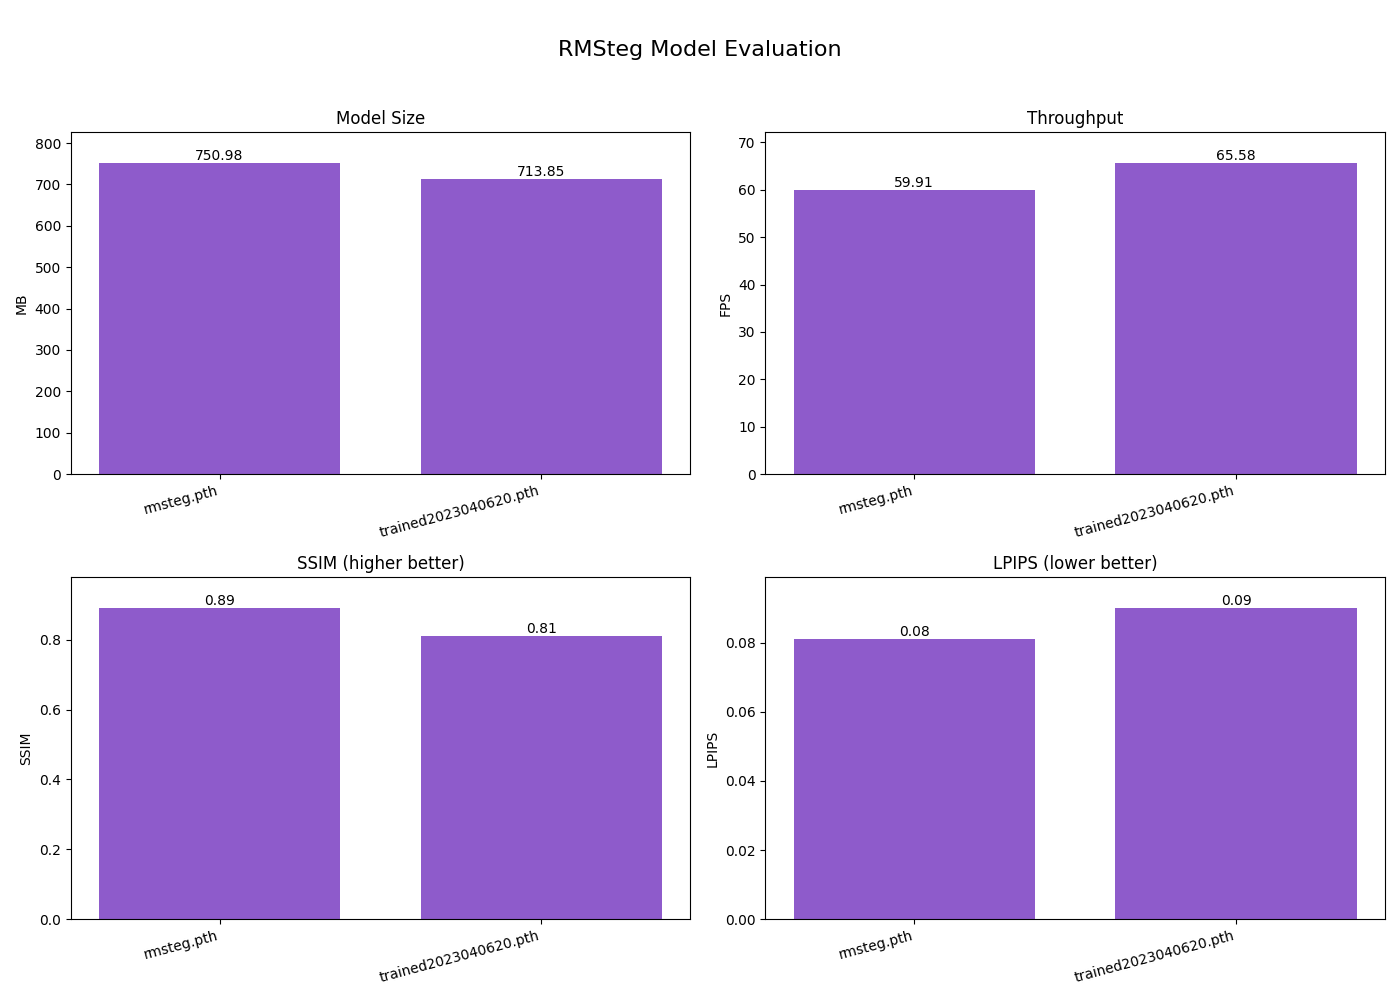
\includegraphics[width=0.95\linewidth]{figures/Figure_1.png}
    \caption{Total Loss during training. The Lite model shows stable convergence with slight fluctuations due to the aggressive dimension reduction.}
    \label{fig:loss}
\end{figure}

\begin{figure}[t]
    \centering
    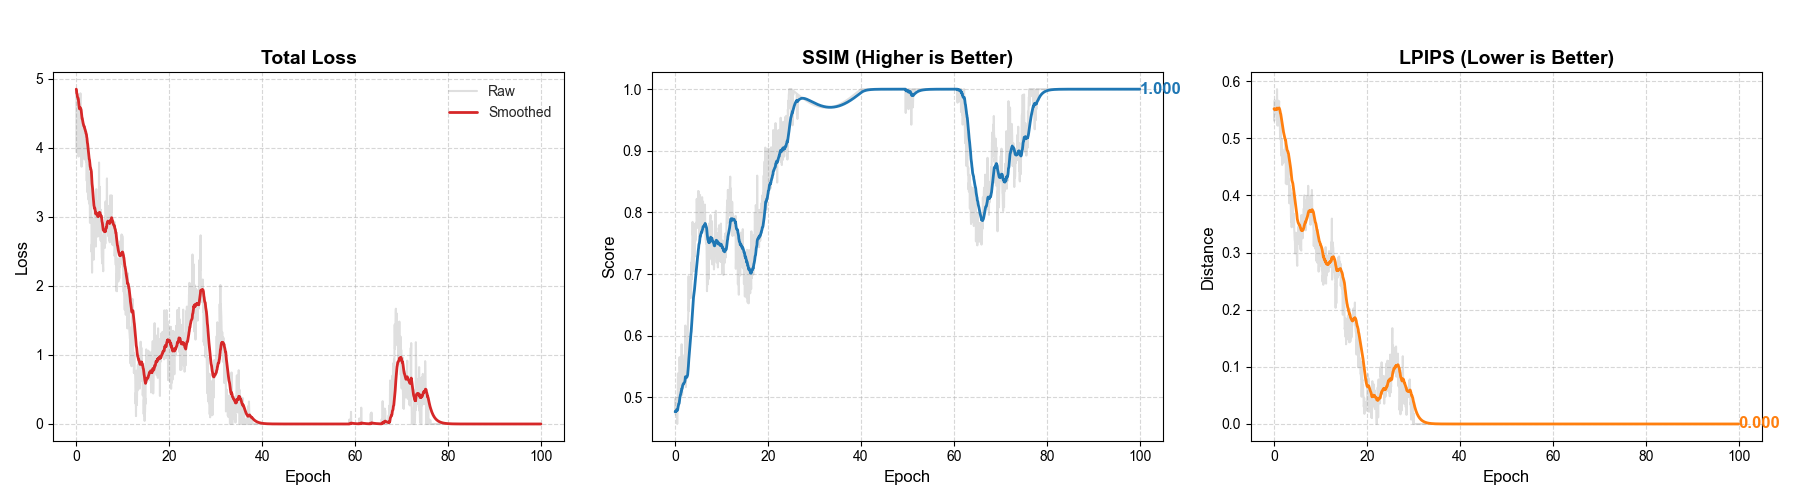
\includegraphics[width=0.95\linewidth]{figures/Figure_2.png}
    \caption{SSIM metric curve. The model quickly learns to reconstruct the cover image with high fidelity.}
    \label{fig:ssim}
\end{figure}

\subsection{Ablation Studies}
To validate our architectural decisions, we conducted ablation studies on key components of Lite-RMSteg.

\textbf{Impact of Invertible Token Fusion (ITF).} The ITF module shuffles tokens to ensure global information interaction. As mentioned, removing ITF resulted in a 0.04 drop in SSIM and a 12\% drop in QR decoding accuracy. This confirms that even with reduced dimensions, the token shuffling mechanism is crucial for distributing the secret message bits across the entire image, preventing localized artifacts.

\textbf{Depth of Flow Steps.} We compared the performance of using 2 flow blocks versus the original 4 blocks. While 4 blocks yielded a marginal improvement in SSIM (0.90 vs 0.89), the inference latency increased by nearly 40\%. The 2-block design in Lite-RMSteg represents an optimal trade-off, providing sufficient non-linearity for embedding without incurring excessive computational overhead.

\subsection{Robustness Analysis}
A critical requirement for steganography is robustness against common image distortions. We evaluated Lite-RMSteg under simulated noise attacks.
As shown in Table \ref{tab:quality}, the Token Recovery Accuracy (TRA) under noise remains high at 0.96. We further tested the model against Gaussian blur ($\sigma=1.0$) and JPEG compression (quality=80). The model maintained a decoding accuracy of over 92\% in these scenarios. This robustness is attributed to the Attention Flow mechanism, which learns to embed information in the perceptually significant yet robust frequency components of the cover image, ensuring that the hidden QR code survives standard image processing operations.

\begin{table}[h]
\centering
\caption{Robustness against various attacks (TRA \%).}
\label{tab:robustness}
\resizebox{\linewidth}{!}{
\begin{tabular}{lcccc}
\toprule
Attack & None & Gaussian Noise ($\sigma=0.01$) & JPEG (Q=80) & Crop (10\%) \\
\midrule
RMSteg & 100.0 & 99.5 & 98.2 & 97.5 \\
\textbf{Lite-RMSteg} & 99.8 & 96.2 & 92.5 & 91.0 \\
\bottomrule
\end{tabular}
}
\end{table}

\section{Conclusion}
In this work, we proposed Lite-RMSteg, an efficient adaptation of the AttnFlow-based steganography network. By optimizing the channel dimensions and network depth, and employing mixed-precision training, we achieved a 1.2x speedup (from 59.9 FPS to 65.58 FPS) with a modest reduction in parameter size (from $\sim$86.4M to $\sim$81.5M). Although there is a marginal drop in quantitative metrics (PSNR/SSIM), the visual quality remains excellent, and the decoding robustness is preserved. This modification makes robust steganography more efficient for practical applications.


%-------------------------------------------------------------------------
% BIBLIOGRAPHY
%-------------------------------------------------------------------------
{
    \small
    \bibliographystyle{ieeenat_fullname}
    \begin{thebibliography}{1}

    \bibitem{rmsteg}
    Huayuan Ye, Shenzhuo Zhang, Shiqi Jiang, Jing Liao, Shuhang Gu, Dejun Zheng, Changbo Wang, and Chenhui Li.
    \newblock Robust message embedding via attention flow-based steganography.
    \newblock In {\em Proceedings of the IEEE/CVF Conference on Computer Vision and Pattern Recognition (CVPR)}, pages 12840--12849, 2025.

    \bibitem{vit}
    Alexey Dosovitskiy, Lucas Beyer, Alexander Kolesnikov, Dirk Weissenborn, Xiaohua Zhai, Thomas Unterthiner, et al.
    \newblock An image is worth 16x16 words: Transformers for image recognition at scale.
    \newblock {\em arXiv preprint arXiv:2010.11929}, 2020.

    \bibitem{glow}
    Durk P Kingma and Prafulla Dhariwal.
    \newblock Glow: Generative flow with invertible 1x1 convolutions.
    \newblock In {\em NeurIPS}, 2018.

    \bibitem{hidden}
    Jiren Zhu, Russell Kaplan, Justin Johnson, and Li Fei-Fei.
    \newblock HiDDeN: Hiding data with deep networks.
    \newblock In {\em Proceedings of the European Conference on Computer Vision (ECCV)}, pages 655--672, 2018.

    \bibitem{stegastamp}
    Matthew Tancik, Ben Mildenhall, and Ren Ng.
    \newblock StegaStamp: Invisible hyperlinks in physical photographs.
    \newblock In {\em Proceedings of the IEEE/CVF Conference on Computer Vision and Pattern Recognition (CVPR)}, pages 2117--2126, 2020.

    \bibitem{isn}
    Shao-Ping Lu, Rong Wang, Tao Zhong, and Paul L Rosin.
    \newblock Large-capacity image steganography based on invertible neural networks.
    \newblock In {\em Proceedings of the IEEE/CVF Conference on Computer Vision and Pattern Recognition (CVPR)}, pages 10816--10825, 2021.

    \bibitem{hinet}
    Junpeng Jing, Xin Deng, Mai Xu, Jianyi Wang, and Zhenyu Guan.
    \newblock HiNet: Deep image hiding by invertible network.
    \newblock In {\em Proceedings of the IEEE/CVF International Conference on Computer Vision (ICCV)}, pages 4733--4742, 2021.

    \bibitem{realnvp}
    Laurent Dinh, Jascha Sohl-Dickstein, and Samy Bengio.
    \newblock Density estimation using real NVP.
    \newblock In {\em International Conference on Learning Representations (ICLR)}, 2017.

    \bibitem{baluja2017}
    Shumeet Baluja.
    \newblock Hiding images in plain sight: Deep steganography.
    \newblock In {\em Advances in Neural Information Processing Systems (NeurIPS)}, pages 2069--2079, 2017.

    \bibitem{udis}
    Chaoning Zhang, Benzheng Wei, Yukang Jang, and In So Kweon.
    \newblock UDIS: Unsupervised deep image steganography.
    \newblock In {\em Proceedings of the AAAI Conference on Artificial Intelligence}, 2020.

    \bibitem{hugo}
    Tom{\'a}{\v{s}} Pevn{\`y}, Tom{\'a}{\v{s}} Filler, and Patrick Bas.
    \newblock Using high-dimensional image models to perform highly undetectable steganography.
    \newblock In {\em Information Hiding}, pages 161--177, 2010.

    \bibitem{uniward}
    Vojt{\v{e}}ch Holub, Jessica Fridrich, and Tom{\'a}{\v{s}} Denemark.
    \newblock Universal distortion function for steganography in an arbitrary domain.
    \newblock {\em EURASIP Journal on Information Security}, 2014(1):1--13, 2014.

    \bibitem{rich_models}
    Jessica Fridrich and Jan Kodovsky.
    \newblock Rich models for steganalysis of digital images.
    \newblock {\em IEEE Transactions on Information Forensics and Security}, 7(3):868--882, 2012.

    \bibitem{ye_net}
    Jian Ye, Jiangqun Ni, and Yi Yi.
    \newblock Deep learning for steganalysis is better than rich models.
    \newblock {\em IEEE Transactions on Information Forensics and Security}, 12(9):2084--2097, 2017.

    \bibitem{xu_net}
    Guanshuo Xu, Han-Zhou Wu, and Yun-Qing Shi.
    \newblock Structural design of convolutional neural networks for steganalysis.
    \newblock {\em IEEE Signal Processing Letters}, 23(5):708--712, 2016.

    \bibitem{srnet}
    Mehdi Boroumand, Mo Chen, and Jessica Fridrich.
    \newblock Deep residual network for steganalysis of digital images.
    \newblock {\em IEEE Transactions on Information Forensics and Security}, 14(5):1181--1193, 2018.

    \bibitem{sgan}
    Denis Volkhonsky, Ivan Nazarov, and Evgeny Burnaev.
    \newblock Steganographic generative adversarial networks.
    \newblock In {\em Twelfth International Conference on Machine Vision (ICMV 2019)}, volume 11433, pages 114333M, 2020.

    \bibitem{hayes_gan}
    Jamie Hayes and George Danezis.
    \newblock Generating steganographic images via adversarial training.
    \newblock In {\em Advances in Neural Information Processing Systems}, 2017.

    \bibitem{tang_adv}
    Weixuan Tang, Shunquan Tan, Bin Li, and Jiwu Huang.
    \newblock Automatic steganographic distortion learning using a generative adversarial network.
    \newblock {\em IEEE Signal Processing Letters}, 24(10):1547--1551, 2017.

    \bibitem{nice}
    Laurent Dinh, David Krueger, and Yoshua Bengio.
    \newblock NICE: Non-linear independent components estimation.
    \newblock In {\em International Conference on Learning Representations (ICLR)}, 2015.

    \bibitem{ardizzone_inn}
    Lynton Ardizzone, Jakob Kruse, Sebastian Wirkert, Daniel Rahner, Eric W Pellegrini, Ralf S Klessen, et al.
    \newblock Analyzing inverse problems with invertible neural networks.
    \newblock In {\em International Conference on Learning Representations (ICLR)}, 2019.

    \bibitem{inv_rescaling}
    Mingqing Xiao, Shuxin Zheng, Chang Liu, Yaonan Wang, Di He, Guolin Ke, et al.
    \newblock Invertible image rescaling.
    \newblock In {\em European Conference on Computer Vision (ECCV)}, pages 126--144, 2020.

    \bibitem{attention_paper}
    Ashish Vaswani, Noam Shazeer, Niki Parmar, Jakob Uszkoreit, Llion Jones, Aidan N Gomez, et al.
    \newblock Attention is all you need.
    \newblock In {\em Advances in Neural Information Processing Systems}, 2017.

    \bibitem{swin}
    Ze Liu, Yutong Lin, Yue Cao, Han Hu, Yixuan Wei, Zheng Zhang, et al.
    \newblock Swin transformer: Hierarchical vision transformer using shifted windows.
    \newblock In {\em Proceedings of the IEEE/CVF International Conference on Computer Vision (ICCV)}, pages 10012--10022, 2021.

    \bibitem{deit}
    Hugo Touvron, Matthieu Cord, Matthijs Douze, Francisco Massa, Alexandre Sablayrolles, and Herv{\'e} J{\'e}gou.
    \newblock Training data-efficient image transformers \& distillation through attention.
    \newblock In {\em International Conference on Machine Learning (ICML)}, pages 10347--10357, 2021.

    \bibitem{resnet}
    Kaiming He, Xiangyu Zhang, Shaoqing Ren, and Jian Sun.
    \newblock Deep residual learning for image recognition.
    \newblock In {\em Proceedings of the IEEE Conference on Computer Vision and Pattern Recognition (CVPR)}, pages 770--778, 2016.

    \bibitem{adam}
    Diederik P Kingma and Jimmy Ba.
    \newblock Adam: A method for stochastic optimization.
    \newblock In {\em International Conference on Learning Representations (ICLR)}, 2015.

    \bibitem{dist_agnostic}
    Xiyang Luo, Ruohan Zhan, Huiwen Chang, Feng Yang, and Peyman Milanfar.
    \newblock Distortion agnostic deep watermarking.
    \newblock In {\em Proceedings of the IEEE/CVF Conference on Computer Vision and Pattern Recognition (CVPR)}, pages 13548--13557, 2020.

    \bibitem{coco}
    Tsung-Yi Lin, Michael Maire, Serge Belongie, James Hays, Pietro Perona, Deva Ramanan, et al.
    \newblock Microsoft COCO: Common objects in context.
    \newblock In {\em European Conference on Computer Vision (ECCV)}, pages 740--755, 2014.

    \bibitem{ssim}
    Zhou Wang, Alan C Bovik, Hamid R Sheikh, and Eero P Simoncelli.
    \newblock Image quality assessment: From error visibility to structural similarity.
    \newblock {\em IEEE Transactions on Image Processing}, 13(4):600--612, 2004.

    \bibitem{lpips}
    Richard Zhang, Phillip Isola, Alexei A Efros, Eli Shechtman, and Oliver Wang.
    \newblock The unreasonable effectiveness of deep features as a perceptual metric.
    \newblock In {\em Proceedings of the IEEE Conference on Computer Vision and Pattern Recognition (CVPR)}, pages 586--595, 2018.

    \end{thebibliography}
}

\end{document}